\chapter{Analysis and Discussion}\label{discussion}
This chapter will summarize the key findings presented in~\Cref{experiments} and analyze them with respect to the theory as outlined in~\Cref{background}. The chapter will be organized according to the experiments performed, with each section discussing the results, impact, and limitations of the corresponding experiment, as well as highlighting potential improvements to the corresponding method(s). The chapter will start with the results from the individual experiments, including the impact of model architectures on generalization as presented in~\Cref{models}, the impact of augmentation as presented in~\Cref{augmentations}, inconsistency Training as presented in~\Cref{consistency_training}, and finally ensembles as presented in~\Cref{ensembles}. Afterwards, the generalizability of the best performing configuration tested in this thesis will be discussed and considered from a practical perspective.
% Finally, the last section will discuss miscellaneous ideas for directions of further research on generalizability which due to a variety of reasons were not explored in this thesis. 

\section{Model Architectures and Generalizability}\label{discussion:models}
The experiments performed in~\Cref{models} show that every model exhibited comparable levels of generalisation failure, with the exception of TriUnet which seemed to struggle more than any of the other models. On Etis-LaribDB, which evidently proved to be the most difficult dataset, every model exhibited a generalizability gap of at least around 50\%, with the TriUnet ranging upwards of 65\%. The degree of generalization failure was slightly less pronounced on the two other datasets, with CVC-ClinicDB exhibiting average gaps of approximately 18\% and EndoCV2020 25\%. 

The models exhibited comparable performance also in \gls{ind} settings, spanning between IoUs of 0.819 and 0.832, which for practical purposes can be considered negligible. 

\subsection{Impact}
Naturally, deploying any of the predictors from this experiment in a clinical setting would be inadvisable and perhaps even harmful. Even if the predictors were to be trained on a dataset collected exclusively from the centre they were intended to be deployed on, there is no guarantee that there would never be some form of distributional shift, which as evidenced by the results significantly affect performance. This distributional shift may be as simple as a change in endoscopy preparation routines, or perhaps an upgrade to a higher resolution cameras, and so on. As established in~\Cref{background}, a system based on models with this lack of generalizability would be practically useless. 

Moreover, these results highlight that researching the development of more and more complicated task-agnostic models is a comparatively fruitless affair. The difference between DeepLabV3+ and Unet - which are separated by two years of research - are practically inconsequential. Admittedly, the differences are more pronounced when the models are trained according to the more sophisticated training regiments used in the remaining experiments, but it is nonetheless clear that it is not advancement in model architectures that is likely to result in increased generalization, but rather improvements to the pipeline with which they are trained.

\subsection{Dual Decoder Models}
\Cref{methods} introduced the dual-decoder DeepLabV3+, the intent of which was to increase generalization by constraining the space of latent representations that the model could leverage, thus in theory mitigating underspecification. As the results in~\Cref{dd-deeplab} showed, however, the effect of this additional encoder was fairly limited when compared to the regular DeepLabV3+. Though it was argued that the reduced performance variability of the dual-decoder model could be interpreted as evidence for a reduction in underspecification, the performance in terms of mean IoU was identical across both models for practical purposes. It was hypothesized that this may be due to the encoder learning principally dataset-agnostic features and consequently primarily performing image compression regardless of what object the model is intended to segment. This was to some extent was corroborated by the analysis performed in~\Cref{dd-deeplab}, which showed equivalent image reconstruction performance across datasets in terms of L1 distance. Further research is however required, as these findings are only representative of one specific model trained in a limited number configurations. One possible direction is to implement a wide range of encoder-decoder models trained across multiple decoder configurations and datasets, and then investigate the latent spaces of the resulting predictors. If the predictor encoders indeed do encode primarily dataset-agnostic features independent of the decoder function, one would expect that one could simply switch encoders between predictors trained on different datasets, domains and tasks without significant performance degradation. 

This behaviour may also be attributed to pretraining. Since the models used throughout this thesis were at least partially pretrained on Imagenet, it might simply be the case that the encoders have learned to perform image compression as a direct consequence of the fact that this likely is the most conducive configuration to minimizing risk on the Imagnet dataset. In this case, the encoder may be in such a wide minimum that actually learning domain-specific features is unlikely even after training to segment polyps. This will be discussed further in~\Cref{pretraining}.


\section{Data Augmentation and Generalizability}
The experiment in~\Cref{augmentations} demonstrated the efficacy of data augmentation as a means of increasing generalization, with IoU improvements on Etis-LaribDB averaging about 15\% and ranging upwards of 30\% when compared to the pipeline without data augmentation. This, as mentioned in~\Cref{background}, can be attributed to the increase in support that the wider diversity of data provides. 

\subsection{Impact}

What is surprising is the extent to which augmentation improves generalization in comparison to some of the other tested methods. In particular, the effects of model architectures and ensembles were both comparatively minuscule. The use of ensembles, for instance, the use of which was the basis of several of the papers submitted to EndoCV2021, increased generalization by at most \(4.81\%\) and on average \(2.65\%\).  The use of data augmentation led to increases of at most \(19.57 \%\) and on average \(8.99\%\) when compared to no augmentation. and Consistency Training at most \(26.07\%\) and on average \(11.73\%\). What this means, in effect, is that the margins by which the use of augmentation affects generalization are far greater than the margins by which ensembles and perhaps many of the other methods presented in EndoCV2021 affect generalization. This raises questions as to the validity of the results in EndoCV2021, which did not control for the choice of data augmentations when comparing submissions. It may, for instance, be the case that certain submissions exhibited high degrees of generalization not strictly because of the impact of their proposed methods, but rather due to their choice of augmentations. This is of course not a certainty, and does as such warrant further research for instance in the form of a meta-analysis. 

\subsection{Inpainting and Generative Modelling}

The experiments in~\Cref{augmentations} showed that the use of an inpainter as implemented in this thesis harmed generalization when used in conjunction with conventional augmentations. Two hypotheses for why this is the case were suggested - either the inpainter simply does not perform to a sufficient standard conducive for use as augmentation, or the inpainter learned the distribution to such an extent that it increased the models' dataset bias. 

To investigate this, it is possible to implement one of the more state-of-the-art inpainting architectures, for instance an inpainting generative multi-column network \cite{inpainter_better}. Additionally, analyzing the generated polyps via statistical means may also have some merit. The development of distance metrics to facilitate easier comparison between synthetic images to real images may for instance be worth looking into, as this might shed some light on the hypotheses as presented above.

\subsection{Limitations}
    Ignoring the inpainter and its flaws as outlined above, only one implementation of data augmentation was used throughout this thesis. The constituent transformations and the values of the hyperparameters thereof were also selected with limited prototyping or testing. There may as such be augmentation configurations that induce significantly increased generalization. By the same token, the selection of transformations used in this thesis may instead have been lucky and thus over-represent the typical contribution of data augmentation. A robust investigation of data augmentation and its effects would require a larger range of augmentation strategies. The results thereof would, however, only be of relevance to the particular task that is being considered. Polyp segmentation may benefit more from augmentation than image-captioning, for instance. 
    
    Additionally, the augmentations in this thesis were applied according to a predetermined probability. A more effective technique may be to augment every sample, but account for the severity through the modulation of the hyperparameters of the constituent transformations. This was not, however, investigated in this thesis, as the probability-based implementation facilitated more apples-to-apples comparison to Consistency Training. 

\section{Consistency Training and Generalizability}
Consistency training was shown to improve generalizability, outperforming data augmentation by a significant margin on Etis-LaribDB. As discussed in~\Cref{methods}, this can be attributed to the fact that, in addition to increasing the models' support, similar to data augmentation, it also imposes more credible inductive biases by explicitly optimizing for consistency across augmentations. 

% \subsection{Mathematical Analysis of Consistency Training}
% The relationship between Consistency Training and conventional data augmentation may be more readily understood mathematically. As mentioned in~\Cref{methods}, one can argue that they may be equivalent, but as the analysis below will show, this is not the case. To illustrate, consider the impact of the respective methods on the gradients. As discussed in~\Cref{background}, the gradient simply defines a direction in the search landscape, and thus if it can be proved that the gradients are not equal (up to scale), it follows that the training process will explore different parts of the search-landscape, irrespective of any amount of tuning of learning rates or any of the other hyperparameters governing the optimization process. 

% As \gls{sil} is based in part on the Jaccard index, it will be compared to a pipeline that uses the Jaccard loss. Moreover, since data augmentation is a stochastic process - in other words, the augmentations applied according to some probability \(p\), the gradients can only be analyzed sufficiently by considering the expected loss. 
% \begin{align*}
%     \mathcal{L} &= \mathbb{E}_p[\mathcal{J}(Z)]; Z \in_{R \thicksim p} \{ \{y, \hat{y}\},\{a, \hat{a}\}\\
%     &= p\mathcal{J}(a, \hat{a})+ (1-p)\mathcal{J}(y, \hat{y})
% \end{align*}
% Thus, the expected gradient is simply:
% \begin{equation}
%     \nabla \mathcal{L} = p \nabla \mathcal{J}(a, \hat{a})+ (1-p)\nabla \mathcal{J}(a, \hat{a})
% \end{equation}
% In the case of \gls{sis}:
% \begin{align*}
%     \bar{\mathcal{C}} &= \sum \frac{\Theta(y, \hat{y},  a, \hat{a})}{\bigcup(y, \hat{y},  a, \hat{a})}\\
%     &= \sum \frac{\bigcup(\Theta(y, \hat{y}), \Theta(a, \hat{a}))- \bigcap (\Theta(y, \hat{y}), \Theta(a, \hat{a})) }{\bigcup(y, \hat{y},  a, \hat{a})}
%     &=...\\
%     \nabla \bar{\mathcal{C}} &=\frac{\mathrm{\nabla_{f}}\! \left(\Theta(y, \hat{y}) \right) \Theta(a, \hat{a})}{-\Theta(y, \hat{y}) \Theta(a, \hat{a}) +\Theta(a, \hat{a}) +\Theta(y, \hat{y})}+\\
%     &\frac{\Theta(y, \hat{y}) \mathrm{\nabla_{f}}\! \left(\Theta(a, \hat{a}) \right)}{-\Theta(y, \hat{y}) \Theta(a, \hat{a}) +\Theta(a, \hat{a}) +\Theta(y, \hat{y})}-\\&\frac{\Theta(y, \hat{y}) \Theta(a, \hat{a}) \left(-\mathrm{\nabla_{f}}\! \left(\Theta(y, \hat{y}) \right) \Theta(a, \hat{a}) -\Theta(y, \hat{y}) \mathrm{\nabla_{f}}\! \left(\Theta(a, \hat{a}) \right)+\mathrm{\nabla_{f}}\! \left(\Theta(a, \hat{a}) \right)+\mathrm{\nabla_{f}}\! \left(\Theta(y, \hat{y}) \right)\right)}{\left(-\Theta(y, \hat{y}) \Theta(a, \hat{a}) +\Theta(a, \hat{a}) +\Theta(y, \hat{y}) \right)^{2}}
% \end{align*}
% At this point, the expression is a bit unwieldy. However, it is worth noting that 
% TODO: finish typesetting remainding proof

% The gradients for the respective methods can then be expressed as follows:
% \begin{align}
%     \nabla \bar{C} &= \\
%     \nabla A &= \\
% \end{align}
% Though both are indeed merely weighted sums of the Jaccard losses for the augmented and unaugmented sets, the difference in how they are weighed is key. In contrast to conventional data augmentation, Consistency Training adjusts the loss dynamically according to segmentation performance. This fact may be used to facilitate the implementation Consistency Training also on other domains than segmentation, by instead modifying augmentation probabilities dynamically. This is left as a point of further research, along with investigating other improvements to Consistency Training as will be outlined in the following section. 


        
    \subsection{Impact}
    Though Consistency Training did increase generalization by a considerable amount, the \gls{ood} performance is nevertheless insufficient for practical purposes. The best performance on Etis-LaribDB with Consistency Training was after all merely 0.504, as shown in~\Cref{tab:consistency}. This kind of performance would naturally be of limited utility in clinical applications.
    
    Consistency Training does, however, constitute a step in the right direction. In contrast to competing methods such as Model-Based Robust Deep Learning \cite{modelbased}, Invariant Risk Minimization \cite{IRM}, or multi-domain training \cite{generalization_datamod}, Consistency Training only requires a single dataset, and can as a result be used in practically every segmentation pipeline. The implementation thereof is also conceptually simple, and can for practical purposes be considered a more generalizable alternative to data augmentation. 
    
    Given further development, Consistency Training may prove a promising candidate as a means of alleviating generalization failure to practically viable extents, especially if leveraged in conjunction with other methods. As established in~\Cref{methods}, the limits are in theory only the efficacy of the quantification of consistency for a given task as well as the support provided by the augmentation strategy upon which it is based. Improvements to either of these aspects are likely to contribute to considerable gains in generalizability. 
    
    Developing perturbation models and consistency metrics may also be a great opportunity to incorporate expert input. A clinician could for instance offer insights as to the nature of the perturbations one might expect in practice and thus assist in the development of the perturbation model.
    
\subsection{Limitations}
    During the experiments performed in this thesis, the batch size was set to 8 for all training procedures. As Consistency Training relies on generating pairs of data from a given batch, one may argue that keeping the batch size the same may result in a weak comparison. The experiment should as such ideally be repeated across a number of batch sizes, but this was infeasible due to logistical constraints, in particular with regards to computational resources. 

\subsection{Improving Consistency Training} \label{new_closs}
    As was shown in~\Cref{experiments}, Consistency Training is an effective means of increasing generalization. However, there is still room for further improvement and exploration. For instance, in this thesis consistency was expressed merely as the symmetric difference between the expected change in the output due to augmentation and the actual change due to augmentation. This, however, as discussed in~\Cref{methods}, is largely agnostic to the augmentation being performed. However, the nature of these augmentations should be taken into account. If the image is subjected to a 90 degree rotation, for instance, the prediction would be considered perfectly consistent so long as the pixels corresponding to the polyps are rotated, and the incorrectly classified pixels remain unchanged. However, if the model instead learns to rotate all of the pixels - even those that are incorrectly classified - it may learn a more accurate representation of what constitutes consistent behavior. I.e, instead of expressing inconsistency as:
\begin{equation*}
\mathcal{C}(a, \hat{a},y, \hat{y}) = \frac{\sum\{y \cap a \cap \hat{y} \cap \hat{a} \}}
{\sum\{ y \cup a \cup \hat{y} \cup \hat{a} \}}
\end{equation*}
    One can adjust the expected change term \(a\oplus y\) to \(\hat{y}\oplus \epsilon(\hat{y})\) such that also incorrect predictions can be considered consistent so long as they change in accordance to the nature of the perturbation model \(\epsilon(\cdot)\). The resulting loss function can then be expressed as:
\begin{equation*}
    \bar{\mathcal{C}}(y,a,\hat{y}, \hat{a}) = \sum \frac{\Theta(\hat{y}, \hat{a},  \hat{y}, \epsilon( \hat{y}))}{\bigcup(\hat{y}, \hat{a}, \epsilon(\hat{y})))}
\end{equation*}
Which is equivalent to:
\begin{equation*}
    \bar{\mathcal{C}}(\hat{y}, \hat{a}) = \sum \frac{\Theta(\hat{y}, \hat{a}, \epsilon( \hat{y}))}{\bigcup(\hat{y}, \hat{a}), \epsilon( \hat{y}))}
\end{equation*}
    This also has the advantage of being independent of the labels themselves. This may alleviate complications that may arise as a consequence of poor and/or incomplete labeling which would otherwise affect what the models learn to associate with consistent behaviour. 

    In addition to improving the way by which consistency is quantified, there are several unexplored directions through which the training procedure itself could be further improved. The perturbation model, for instance, could be modified in any number of ways: one could for instance adversarially sample difficult augmentations based on the consistency score, and use these during training. One could also perform a study to ascertain the impact of the perturbation models' constituent augmentation functions on generalization. It may for instance be the case that some of the augmentations used in the perturbation model used in this thesis hampered generalizability more than it facilitated it, though without a complete study this is impossible to say with any certainty.  
    
    One could also experiment with modulating the difficulty of the augmentations. In the experiments performed in this thesis, the augmentation difficulty was kept constant - i.e, the augmentation hyperparameters were capped to a specific range. However, it may be the case that gradually increasing the difficulty or modulate it according to some sort of annealing function could further improve the efficacy of Consistency Training. 
    
    Finally, using multiple perturbed images when computing inconsistency instead of just one may potentially further strengthen the generalizability of the learned features. In this thesis, the inconsistency term really only pertains to the inconsistency of the model with respect to the change being applied to the perturbed input. It is possible to  instead generate multiple perturbed inputs, each being transformed in a different manner, and then compute multiple inconsistency terms thereafter. This does require more memory, however, and may on certain hardware be infeasible unless the batch sizes are kept small. 
    
\section{Ensembles and Generalizability}
    The use of ensembles, as shown in~\Cref{ensembles}, was proved to increase generalization. The improvements were on average comparatively minor, however, with Etis-LaribDB seeing the biggest improvements with an 3.95\% increase in the mean \gls{iou} across models. 
    
    Moreover, the findings as presented in~\Cref{fig:ensemble_var} do to some extent support the hypothesis that this improvement is a consequence of the fact that ensembles mitigate underspecification, as the greatest gains to generalization were achieved by models that initially exhibited high degrees of underspecification as quantified by the performance variability of the respective pipelines. This was not, however, proven with statistical certainty, and requires higher sample sizes and ideally a larger diversity of model-architectures to verify to statistically significant extents.  

    
    \subsection{Impact}
    Though there are gains to be made from the use of ensemble models, it should be noted that ensembles incur higher costs with regards to training time, time required for inference, and memory requirements. This, naturally, needs to be weighted against the benefits, which as discussed are fairly marginal on average. It may, for instance, be the case that the computational resources spent training multiple models for use in an ensemble would be better spent tuning the augmentation strategy, at least if a \gls{ood} dataset is available.
 
    \subsection{Limitations}
    As mentioned in~\Cref{ensembles}, the constituent predictors for each ensemble were sampled from the ten predictors trained for the purpose of the experiments in~\Cref{augmentations} and~\Cref{consistency_training}. As a result, the statistical significance of the findings are not necessarily robust. Thus, the experiments should ideally be repeated with an increased sample size, for instance N=50, such that ten ensembles could be constructed such that each ensemble consists of an independent set of predictors. 
    
    It should also be noted that the experiments in this thesis were performed only at one ensemble size - i.e, five models. This choice was informed by the literature, in particular the implementation of DivergentNet \cite{divergentnets}. Ensembles may as such have a greater impact than expected, dependent on the returns from increasing the model counts. Following the Bayesian perspective as discussed in~\Cref{background:ensembles}, increasing the model count may result in a better estimate of the Bayesian posterior, and thus lead to increased generalization.
    
    The improvements from increasing ensemble size are likely limited. The performance of ensembles is after all bounded by the performance of perfect Bayesian marginalization. As shown in~\Cref{fig:bayesian_generalization}, this will not necessarily constitute perfect generalization, as the predictions are in such a system weighted according to the likelihood that the given weight configuration is returned from the pipeline. Thus, if learning shortcuts is likely, Bayesian marginalization will primarily be predicting according to shortcut features. Investigating this may be an interesting direction of further study.
    
    \subsection{Improving Ensembles through Diversity Search}
    Though ensembles as implemented in this thesis exhibit somewhat limited returns, leveraging a diversity of interpretations of the input data may have considerable merit towards increasing generalization. As the analysis in~\Cref{fig:ensemble_var} shows, there appears to be a positive relationship between generalizability and model-diversity that warrants further investigation. In particular, it may be the case that ensembles consisting of predictors that are trained to explicitly encode differing features are more conducive to generalization than conventionally implemented ensembles. By explicitly optimizing for weight diversity, one might mitigate the tendency of typical ensembles to primarily consider weight configurations that exhibit higher posterior likelihoods. 
    
    This could for instance be achieved by training multiple instances of the same model concurrently, and incorporating model-wise weight variance into the loss function. An illustration of such a pipeline is provided in~\Cref{fig:diversity}.
    
    \begin{figure}[htb]
        \centering
        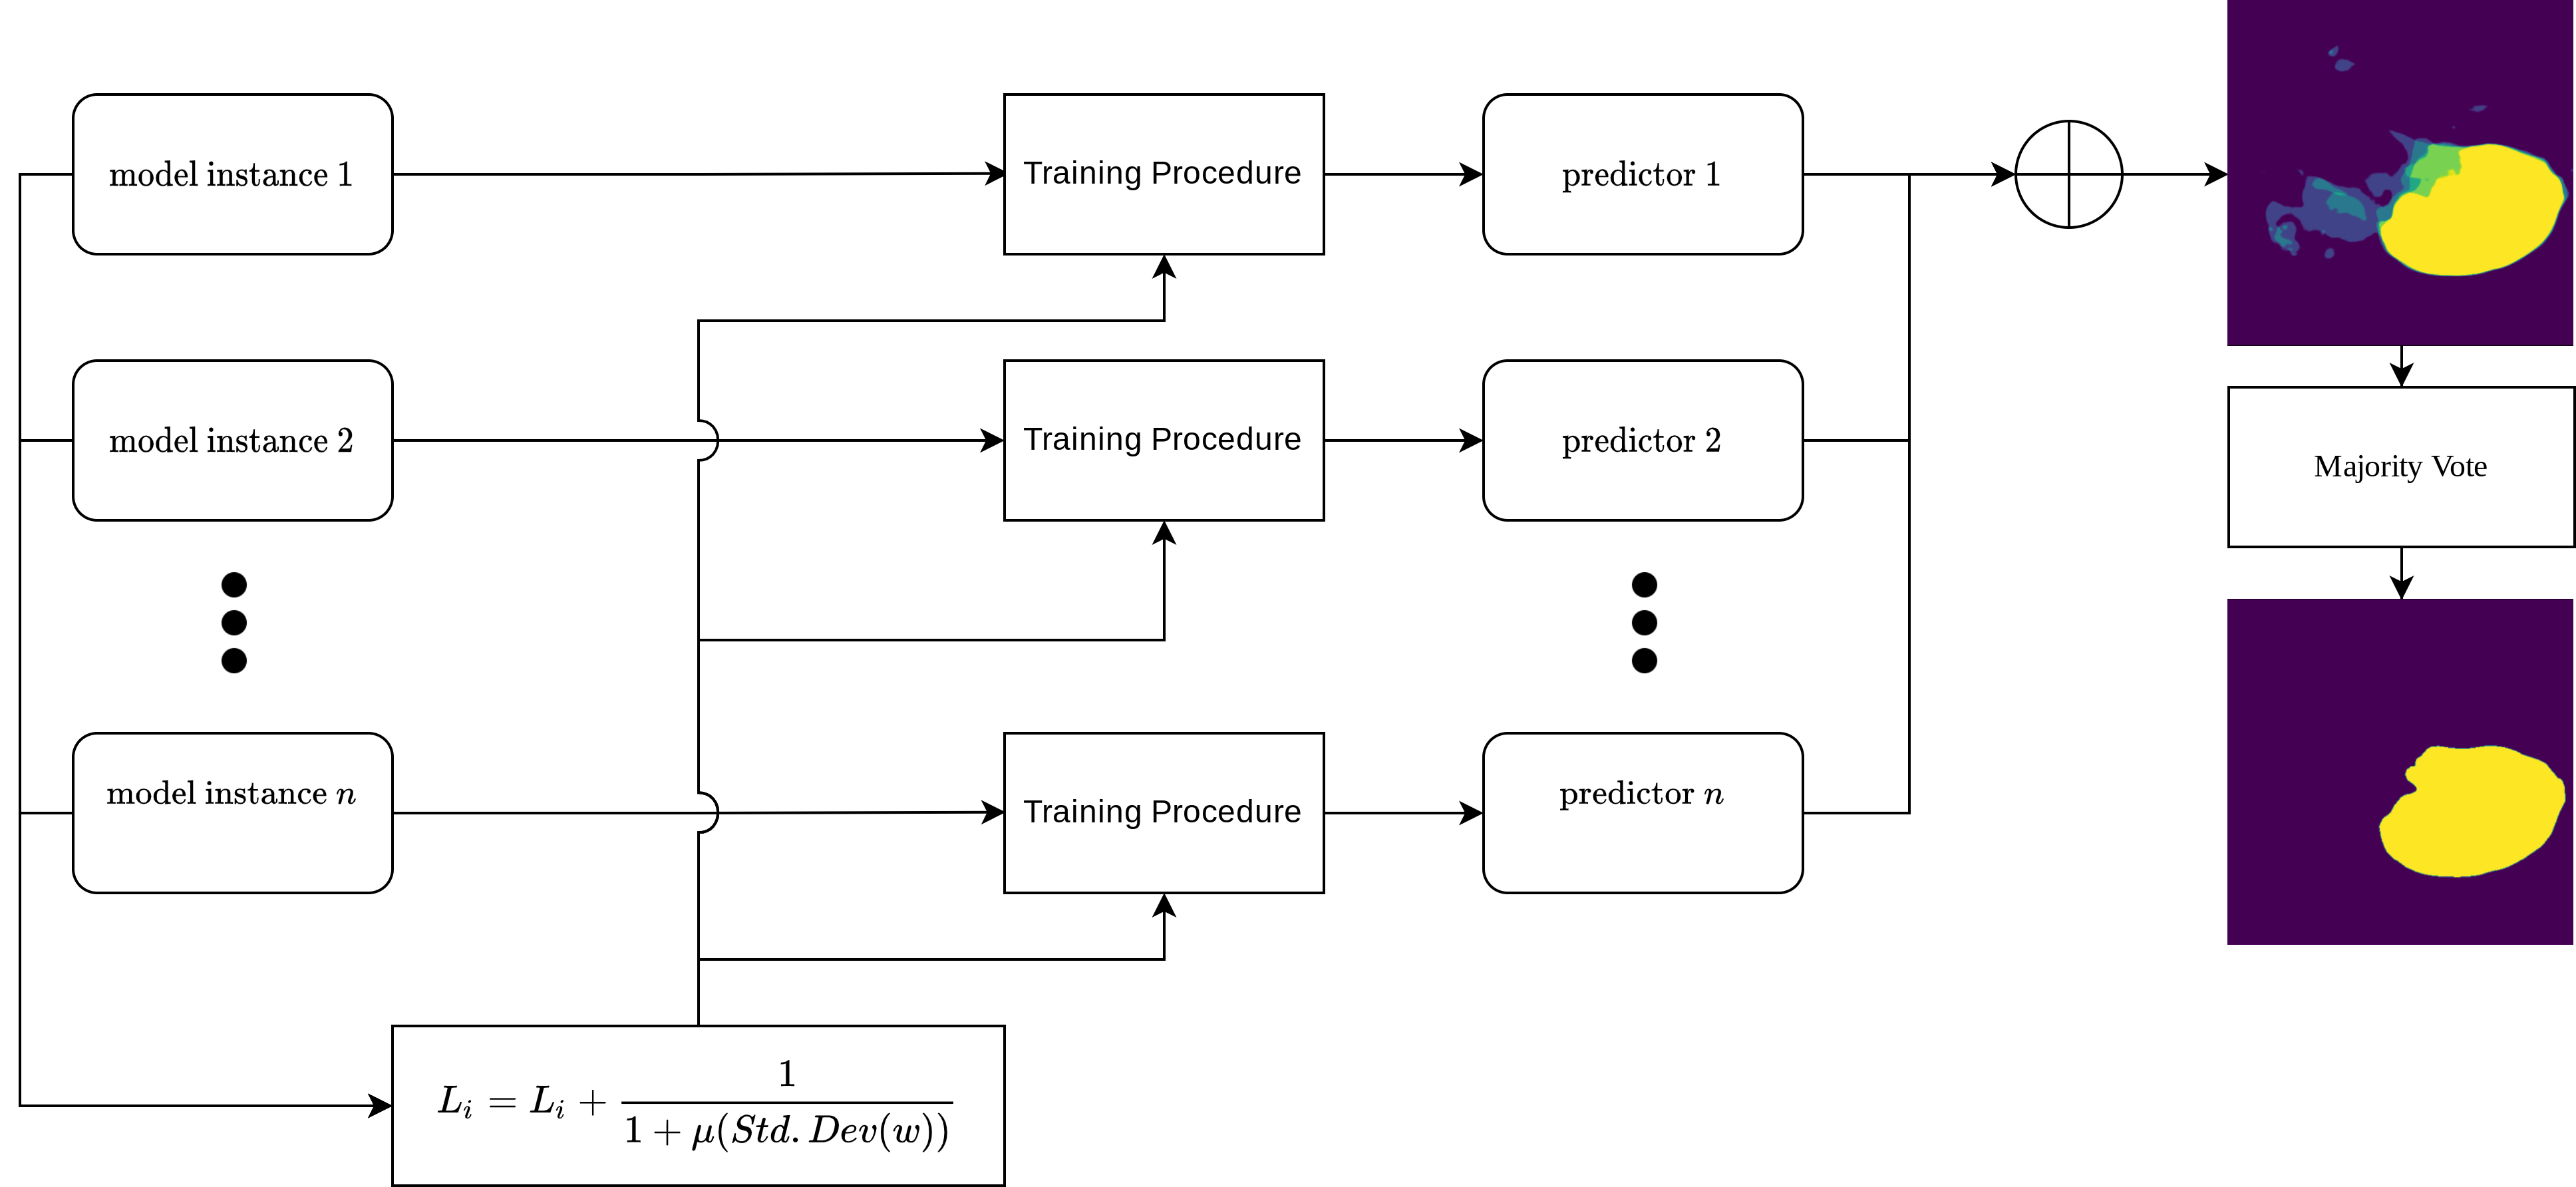
\includegraphics[width=\linewidth]{illustrations/diversity_search.png}
        \caption[Deep Diversity Search]{By adding a term corresponding to the mean standard deviation of weights, the models will learn maximally independent representations, and hence result in predictors with a larger diversity of learned features. This may mitigate underspecification to a greater extent, since this search would be less biased towards regions of the search landscape with high posterior probability.}
        \label{fig:diversity}
    \end{figure}
    
    This way, the ensemble will consist of predictors that encode a wider diversity of interpretations of the data than the predictors in conventional ensembles. This in turn provides a more complete perspective of the many possible interpretations a given model can learn. If this is proven to be the case, using such an ensemble during screening may also actually be viable, as the clinician could then take all of these possible interpretations into account instead of trusting that a single predictor is encoding the right inductive biases.  

\section{Overall Impact}
Though this thesis presents methods that constitute considerable improvements to generalization, the resulting system is nevertheless not particularly useful in practical settings when considered holistically. 

Consider for instance the best performing configuration tested in this thesis, namely the DeepLabV3+ ensemble trained with Consistency Training. This pipeline achieved average \glspl{iou} of 0.751 on CVC-ClinicDB, 0.683 on EndoCV2020, 0.523 on Etis-LaribDB, and 0.859 on Kvasir-SEG. Though this is constitutes a considerable improvement over both of the "naive" pipelines - i.e single models trained with and without regular data augmentation - it is nonetheless not sufficiently generalizable for practical use. Ideally, there should be negligible differences between all four datasets, and though there is some room for some degree of performance degradation, a system that exhibits a mean \gls{iou} of 0.523 is not particularly useful and as discussed in~\Cref{ethics} may actually cause more harm than good. 

Moreover, though Etis-LaribDB was the most difficult of the datasets used in this thesis, the performance on this dataset does not necessarily reflect the worst-case performance in a clinical setting. Indeed, the extent to which the a given pipeline fails to generalize cannot be sufficiently anticipated \cite{trust_ai} given current approaches to deep learning. It may easily be the case that the model performs even worse under certain clinical conditions.

Thus, in spite of the aforementioned improvements, the pipeline as a whole is not in purely practical terms much better than any of the naive pipelines. More work is evidently required to achieve suitable levels of generalization. In addition to the possible improvements for the methods presented in this thesis as discussed in the preceding sections, promising directions of further work will also be outlined in~\Cref{future_work} to this end. 

\section{Summary}
This section presented a more thorough analysis and discussion of the findings as presented in~\Cref{experiments}. The results were analyzed with respect to the literature, the theory as laid out in~\Cref{background}, and considered in terms of viability of clinical deployment. For each experiment, the impact, limitations and potential improvements were discussed where applicable. 

Holistically, the findings in this thesis highlight that generalization remains a challenging problem, but that the development of generalizable methods is an endeavor ripe for further exploration. Consistency Training in particular seems to be a promising candidate for further research towards alleviating generalization failure. It was also shown that further foundational work is required in order to fully understand the relationship between the constituent components of the deep learning pipeline and generalizability, in particular with regards to developing sufficiently well-controlled experimental methodologies and eliminating confounding variables during comparative studies. 